\chapter{中断、异常与系统调用实现}\label{chap:trap-syscall}

中断、异常与系统调用是操作系统内核从“被动等待”转为“响应事件”的核心机制。用户程序通过系统调用主动进入内核，硬件设备通过外部中断通知内核，处理器执行异常则要求内核判断错误来源并采取相应处理。原 IA-32/C++ 版本 Unix V6++ 依赖 IDT、8259A、x86 中断栈帧和多组入口宏完成这些工作；RISC-V/Rust 重构版本则基于 RISC-V 特权架构中的 \verb|stvec|、\verb|sscratch|、\verb|sepc|、\verb|scause|、\verb|stval| 和 \verb|sstatus| 等寄存器重新组织 Trap 框架\cite{riscv_privileged_20211203}。

本章介绍当前系统中 Trap 入口、上下文保存、中断异常分发和系统调用处理的实现。与第 3 章类似，本章也会在关键位置说明重构前后实现方式的差异，并适度分析 Rust 在类型化上下文、模式匹配和错误返回表达上的作用。

\section{Trap 处理总体框架}

RISC-V 将同步异常、异步中断和系统调用统一纳入 Trap 机制。当前系统在初始化阶段调用 \verb|init_trap|，将 \verb|stvec| 设置为 \verb|_trap_entry|，并通过 \verb|sscratch| 绑定当前进程的 \verb|TrapContext| 地址。此后，无论是用户态执行 \verb|ecall|、时钟中断到来，还是用户程序触发非法指令或页面异常，处理器都会跳转到同一个 Trap 入口。

\verb|_trap_entry| 使用裸函数和内联汇编实现。进入 Trap 后，汇编代码首先通过 \verb|csrrw| 交换 \verb|sscratch| 和临时寄存器，使入口代码能够获得当前进程的 \verb|TrapContext| 指针。随后，入口代码依次保存通用寄存器、\verb|sepc|、\verb|scause|、\verb|sstatus|、\verb|stval| 等关键状态。如果 Trap 来自用户态，入口代码还会切换到进程自己的内核栈。保存完上下文后，入口代码调用 Rust 层的 \verb|trap_handler| 完成具体分发；处理结束后再恢复寄存器和控制状态，最后执行 \verb|sret| 返回原执行流。

\begin{figure}[htbp]
  \centering
  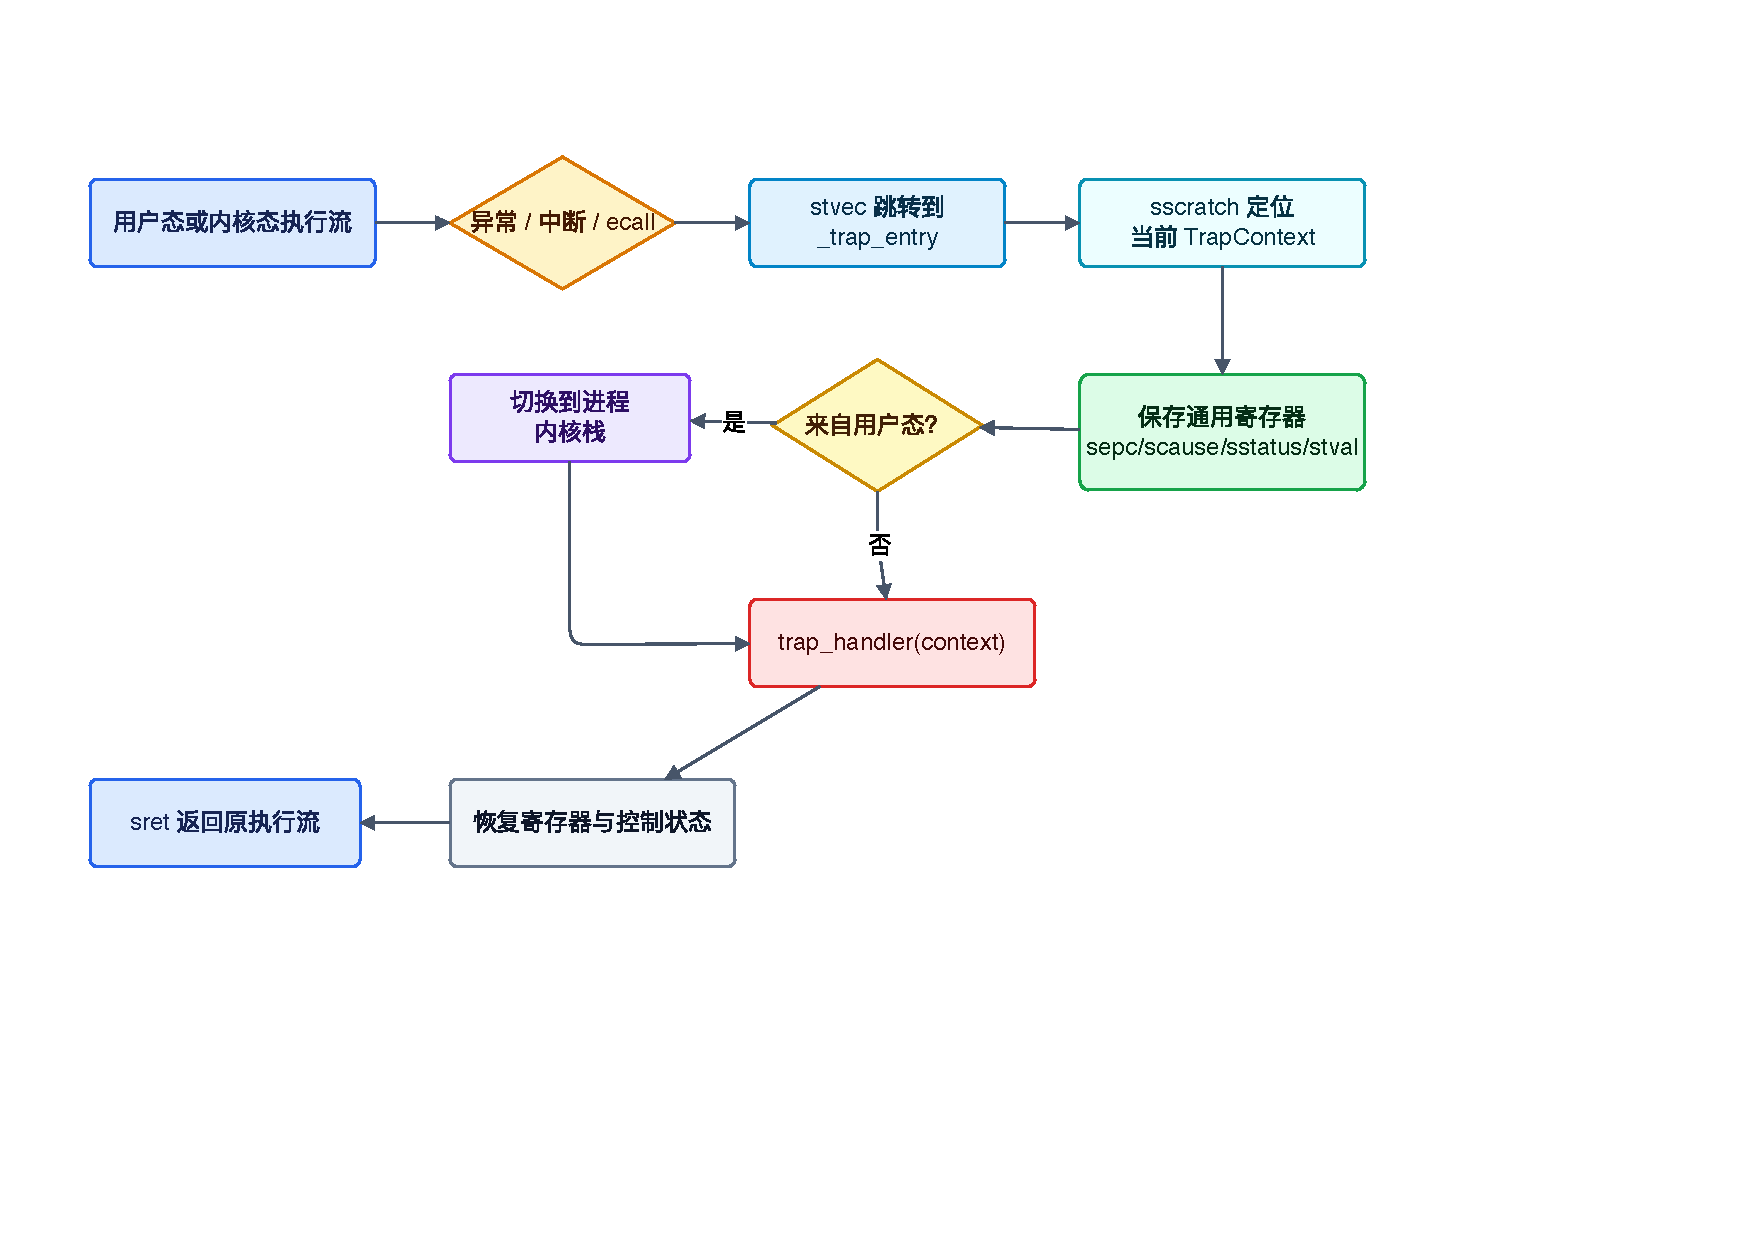
\includegraphics[width=0.95\textwidth]{figures/trap-flow.pdf}
  \caption{RISC-V Trap 入口与返回流程}\label{fig:trap-flow}
\end{figure}

\figref{fig:trap-flow} 展示了这一统一入口的基本路径。该设计与原 IA-32 版本存在明显差异。原版本需要为系统调用、时钟中断、键盘中断和不同异常分别设置 IDT 表项，并在多个入口函数中执行保存现场、切换内核、调用处理函数、恢复现场和 \verb|iret| 返回等步骤。重构后，RISC-V 版本将入口收束到一个 \verb|_trap_entry|，再由 Rust 层根据 \verb|scause| 判断事件类型。这样减少了多处入口代码之间的重复，也使异常、中断和系统调用共享同一份上下文结构。

上下文结构定义在 \verb|src/interrupt/context.rs| 中，包括 \verb|Registers| 和 \verb|TrapContext| 两部分。\verb|Registers| 保存通用寄存器，\verb|TrapContext| 进一步保存 \verb|sstatus|、\verb|sepc|、\verb|scause|、\verb|stval| 和 \verb|kernel_sp|。这些结构使用 \verb|#[repr(C)]| 保证内存布局稳定，并通过 \verb|offset_of!| 生成字段偏移常量，供汇编入口保存和恢复寄存器时使用。这样，汇编代码不需要手写一组与 Rust 结构重复维护的偏移数字，降低了上下文结构调整时产生不一致的风险。

\section{异常与中断分发}

进入 Rust 层后，\verb|trap_handler| 通过 \verb|TrapContext::cause| 读取 \verb|scause| 并分为中断和异常两大类。中断类主要处理 Supervisor Timer 和 Supervisor External；异常类主要处理 Breakpoint、Illegal Instruction、User Environment Call、Instruction/Load/Store Page Fault 以及若干访问异常。Rust 的枚举和模式匹配在这里比较适合表达分发逻辑：代码能够直接按照 \verb|Trap::Interrupt|、\verb|Trap::Exception|、\verb|Interrupt::SupervisorTimer|、\verb|Exception::UserEnvCall| 等分支展开，而不是通过裸整数常量和多层 if 判断完成分发。

\begin{figure}[htbp]
  \centering
  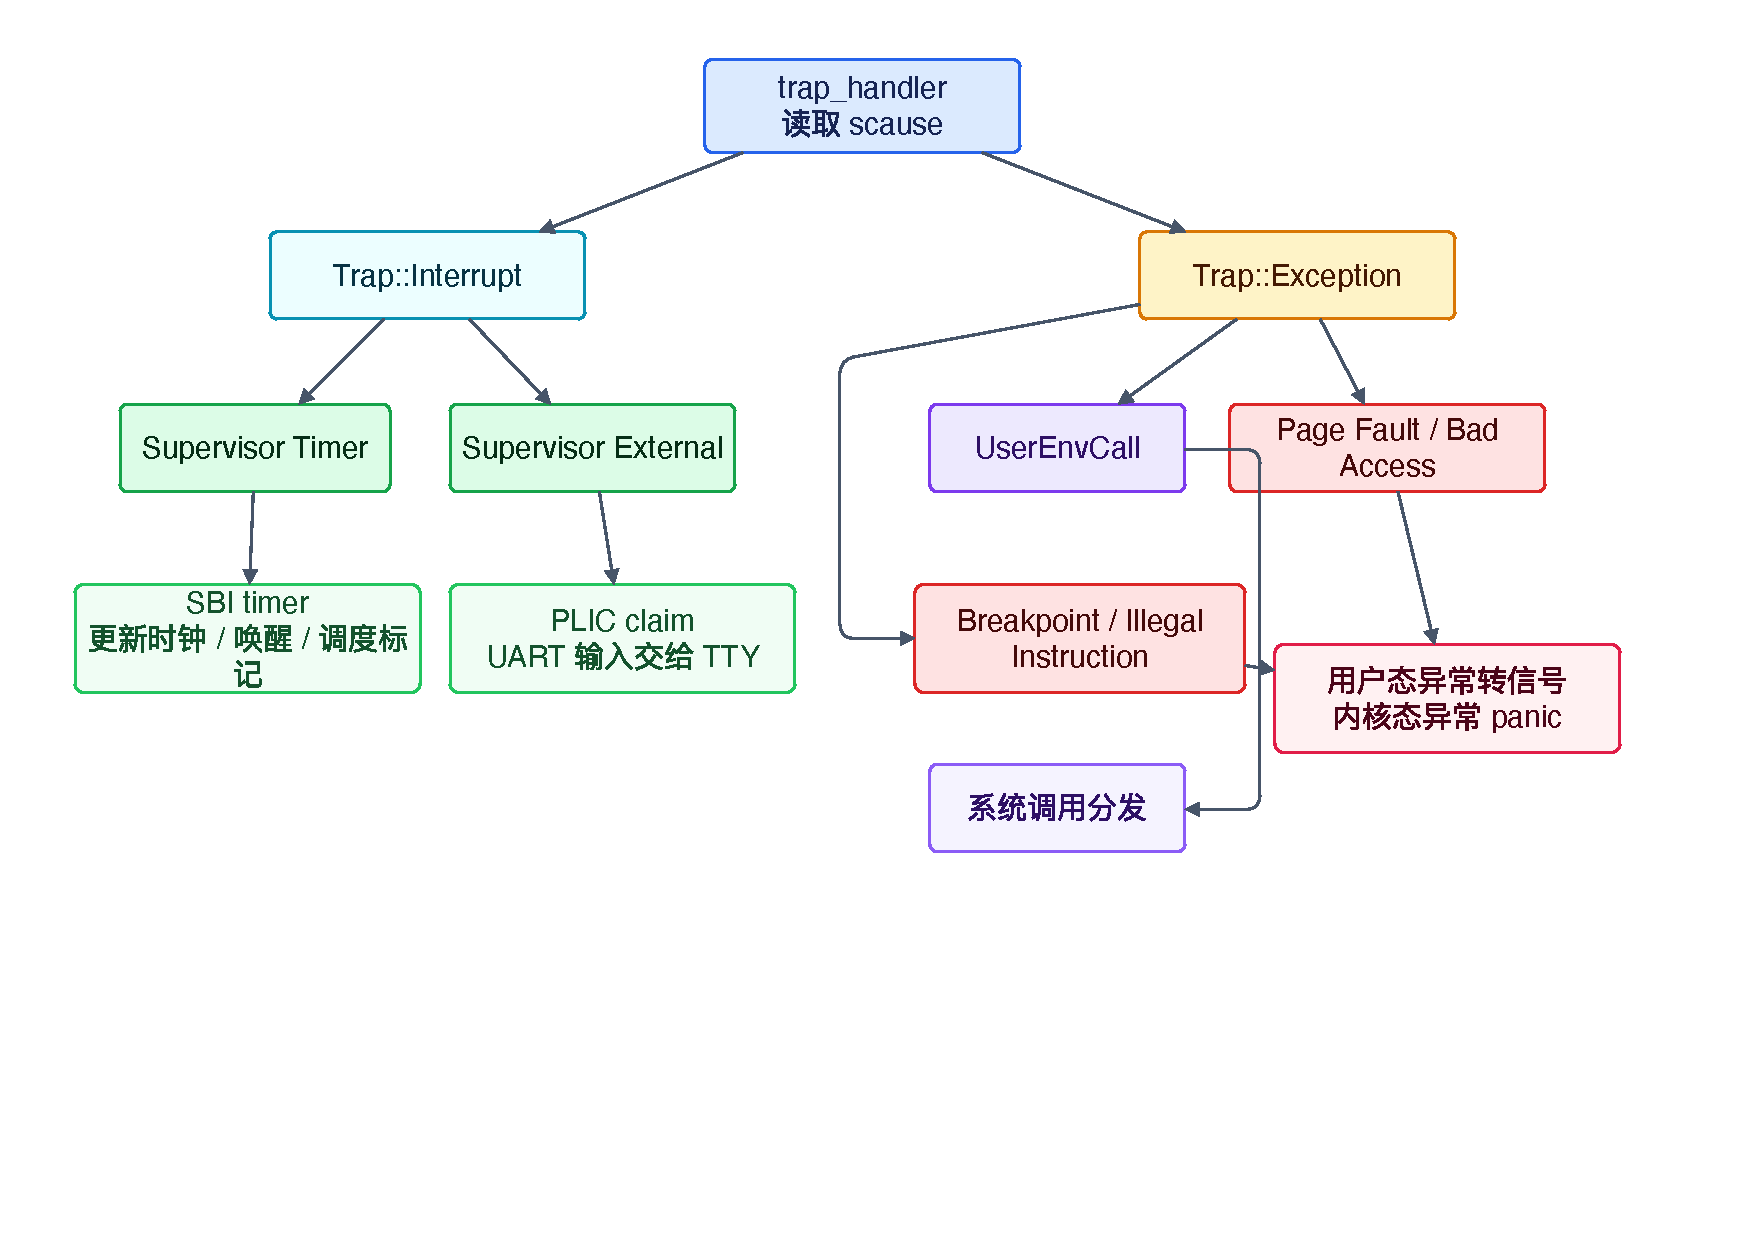
\includegraphics[width=0.95\textwidth]{figures/trap-dispatch.pdf}
  \caption{中断与异常分发路径}\label{fig:trap-dispatch}
\end{figure}

对于时钟中断，系统使用 SBI timer 设置下一次时钟事件。当前实现将每秒中断次数设置为 60 次，定时器中断到来后更新用户态时间或内核态时间，增加当前进程的 CPU 使用计数，并在一秒边界更新系统时间。如果有进程通过 \verb|sleep| 等待某个时间点，系统会在超时后唤醒睡眠队列。时钟中断还会重新计算进程优先级，并在从用户态返回前检查是否需要调度。当前系统不在内核态执行路径中强行抢占，而是在用户态返回边界调用 \verb|schedule_on_user_return|，这与原 Unix 风格“在合适的陷入返回点进行调度”的思路保持一致。

对于外部中断，系统通过 PLIC 进行 claim/complete 操作。当前主要启用 UART0 外部中断：当 PLIC 返回 UART 中断号后，内核从串口读取输入字节，并交给 TTY 层处理。TTY 层再完成回显、行规程和控制字符处理；例如输入中断字符时可以向进程发送相应信号。处理完毕后，内核向 PLIC 写回 complete，表示该中断已经处理结束。与原 IA-32 版本通过 8259A 和键盘中断入口处理输入不同，RISC-V/QEMU virt 版本的输入路径被改写为 UART + PLIC + TTY 的组合。

异常处理则根据异常来源分为可恢复和不可恢复两类。用户态非法指令会被转换为 \verb|SIGILL|，用户态页面异常通常转换为 \verb|SIGSEGV|，访存对齐或总线类错误转换为 \verb|SIGBUS|。如果异常发生在内核态，系统会输出包含 \verb|scause|、\verb|sepc|、\verb|stval| 等信息的 panic 日志并停止。这种处理方式一方面延续了 Unix V6++ 将用户态异常映射为信号的思路，另一方面也利用 RISC-V 的 \verb|stval| 和 \verb|sepc| 信息改善了调试可观察性。

\section{系统调用接口}

系统调用是用户程序主动请求内核服务的主要接口。当前用户态 C 库在 \verb|lib/src/syscall.h| 中封装了 \verb|__syscall0| 到 \verb|__syscall3| 等内联函数。系统调用号放入 \verb|a7|，参数依次放入 \verb|a0|、\verb|a1|、\verb|a2| 等寄存器，随后执行 \verb|ecall| 指令。处理完成后，返回值由内核写回 \verb|a0|。在用户库层，若返回值为负数，则通过 \verb|__syscall_ret| 转换为用户程序习惯的失败返回。

内核收到 \verb|ecall| 后，会在 \verb|trap_handler| 中识别 \verb|Exception::UserEnvCall|，再调用 \verb|system_call::handle_user_ecall|。该函数首先检查当前进程是否有待处理信号；随后将 \verb|sepc| 前进 4 字节，使 Trap 返回后不会再次执行同一条 \verb|ecall|；接着从 \verb|TrapContext| 中取出系统调用参数，写入 Unix V6++ 风格的 \verb|Userspace::args|，并将 \verb|a0| 位置绑定为返回值写入位置。最后，内核按照系统调用号分发到进程管理、文件系统、时间、信号等具体处理函数。

\begin{figure}[htbp]
  \centering
  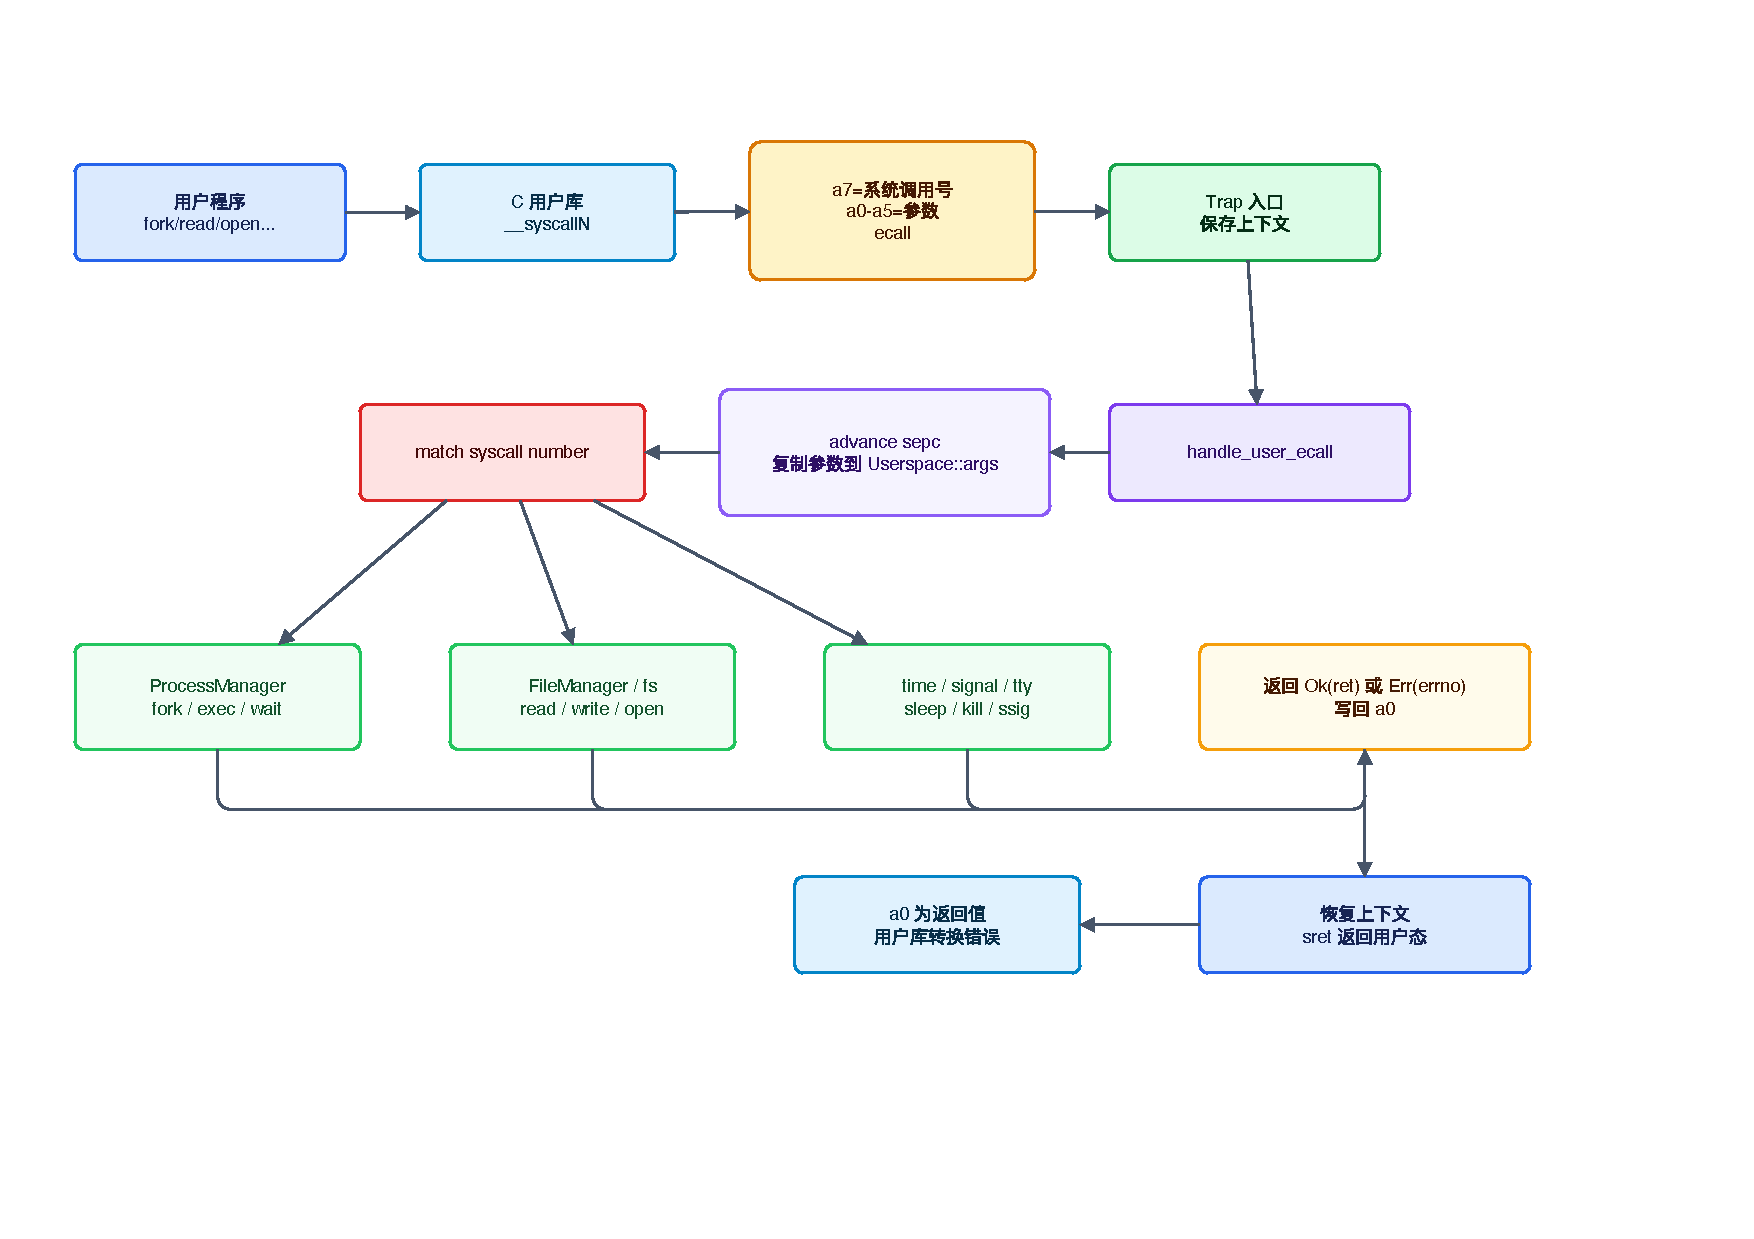
\includegraphics[width=0.95\textwidth]{figures/syscall-path.pdf}
  \caption{用户态到内核态的系统调用路径}\label{fig:syscall-path}
\end{figure}

\figref{fig:syscall-path} 展示了系统调用从用户态 C 库到内核处理函数再返回用户态的路径。当前系统保留了 Unix V6++ 的系统调用编号和主要语义，例如 \verb|exit|、\verb|fork|、\verb|read|、\verb|write|、\verb|open|、\verb|wait|、\verb|exec|、\verb|chdir|、\verb|sleep|、\verb|kill|、\verb|pipe| 和 \verb|signal| 等。部分与当前平台关系不大的调用以空实现或 \verb|ENOSYS| 返回，例如若干未实现编号、\verb|trace| 和部分终端控制调用。这种处理方式有助于保持用户库和 Shell 的接口稳定，同时明确当前系统的功能边界。

与原 IA-32/C++ 版本相比，系统调用分发方式也发生了变化。原版本通过 \verb|SystemCallTableEntry| 表保存参数个数和函数指针，系统调用号来自 \verb|eax|，参数从 \verb|ebx| 等寄存器复制到 \verb|u.u_arg|。RISC-V 版本则使用 \verb|a7| 作为系统调用号，\verb|a0| 到 \verb|a5| 作为最多六个参数，并在 Rust 中通过 \verb|match| 表达分发逻辑。表驱动和模式匹配都能完成系统调用派发；当前版本选择 \verb|match| 的原因在于它与 Rust 的枚举、错误返回和模块函数调用结合更自然，也更容易在编译期检查分支书写是否符合类型约束。

\section{错误返回与信号处理}

系统调用处理中的错误返回沿用了 Unix 风格：内核内部以 \verb|PosixError| 表示错误原因，返回用户态时将错误码取负后写入 \verb|a0|。例如文件描述符无效、权限不足、找不到文件、系统调用未实现等情况都可以通过统一的错误枚举返回。对于仍然沿用原 Unix V6++ 文件系统处理习惯的函数，当前代码提供了 \verb|trap_ret| 和 \verb|trap_void| 包装函数，将 \verb|Userspace::error| 转换为 Rust 的 \verb|KResult|。这样既能复用已有的 Unix V6 风格处理流程，又能让新写的 Rust 代码使用 \verb|Result| 表达成功或失败。

信号处理贯穿异常、终端输入和系统调用返回路径。系统调用进入前，如果当前进程已有待处理信号，内核会优先构造信号处理上下文并返回 \verb|EINTR|；系统调用完成后，内核还会再次检查待处理信号。时钟中断和异常处理也会在合适位置检查当前进程是否需要处理信号。对于用户自定义信号处理函数，内核会保存当前 \verb|TrapContext| 到用户栈，将 \verb|sepc| 改为用户态 handler 地址，并设置返回地址为用户态信号返回跳板。这样，用户程序可以在信号处理函数结束后通过 \verb|sigret| 恢复原先被中断的执行现场。

从 Rust 重构角度看，本部分的主要改进不在于消除所有 unsafe 代码。Trap 入口、用户指针读取、信号上下文压栈和系统调用 ABI 都不可避免地涉及底层内存操作。但重构后的代码将 unsafe 边界集中在少数位置，而将分发、错误转换、信号判断和调度检查放在类型化的 Rust 函数中实现。相比原版本中大量入口宏、寄存器结构和处理函数之间的手工约定，当前实现更容易定位一次 Trap 的完整路径，也更容易在论文和后续实验中解释。

\section{本章小结}

本章介绍了 RISC-V/Rust 版本 Unix V6++ 的中断、异常与系统调用实现。系统通过 \verb|stvec| 建立统一 Trap 入口，使用 \verb|sscratch| 定位当前进程的 \verb|TrapContext|，在汇编层完成寄存器保存与恢复，并在 Rust 层根据 \verb|scause| 进行中断、异常和系统调用分发。时钟中断由 SBI timer 驱动，外部中断由 PLIC 和 UART 输入路径处理，用户态异常则根据类型转换为相应信号。系统调用路径从用户态 C 库的 \verb|ecall| 开始，经过 Trap 入口和 Rust 分发函数，最终调用进程、文件系统、时间和信号等内核模块。

从工作量角度看，本章对应的实现包括：重写 RISC-V Trap 入口汇编，设计 \verb|TrapContext| 与寄存器偏移常量，接入 \verb|stvec|、\verb|sscratch|、SBI timer、PLIC 和 UART 中断，迁移 Unix V6++ 系统调用编号与用户库 ABI，并实现错误返回、信号检查和用户态返回前调度等逻辑。这些工作连接了第 3 章中的内存和页表基础，也为后续进程管理、文件系统和终端交互提供了运行支撑。
